\section{Depth Calibration Framework for the RealSense D435i}

To ensure high-precision localization, the Intel RealSense D435i was calibrated to eliminate systematic depth inconsistencies. The implementation follows a supervised learning approach using polynomial regression to map raw sensor data to true spatial coordinates.

\subsection{Experimental Data Acquisition Strategy}
The calibration environment was designed to capture the "bowl effect" distortion characteristic of stereo-depth sensors. An ArUco marker (Dictionary 8x8/AprilTag) was placed on objects of known heights, verified with a 1 mm resolution metric scale. Data collection was performed using a custom Python-based acquisition script that recorded:
\begin{itemize}
    \item The refined pixel coordinates $(u, v)$ of the marker center.
    \item The raw distance $Z_{meas}$ reported by the RealSense SDK.
    \item The verified ground-truth distance $Z_{true}$.
\end{itemize}
Approximately 500 points were sampled across the entire Field of View (FoV) to ensure the regression model captures radial depth inaccuracies.

\subsection{Polynomial Regression and Temporal Filtering}
A second-order polynomial model was implemented to "flatten" the depth field. The model predicts the corrected depth $Z_{corr}$ as a function of the spatial position and raw depth:
\begin{equation}
Z_{corr} = f(u, v, Z_{meas})
\end{equation}

To mitigate the inherent high-frequency noise of the D435i, a 1D Kalman Filter was integrated into the ROS2 pipeline. This filter utilizes a constant-velocity state-space model to provide a smoothed trajectory of the detected object height.
\clearpage
\subsection{Results and Discussion}

\subsubsection{RealSense Calibration Performance Analysis}

The effectiveness of the depth calibration was evaluated through spatial error mapping and quantitative statistical analysis. 

\subsubsection{Spatial Error Characterization}
Before calibration, the sensor exhibited significant systematic errors increasing towards the image boundaries. Figure~\ref{fig:spatial_comparison} illustrates the transformation from a warped depth field to a homogenized Cartesian plane.

\begin{figure}[H]
    \centering
        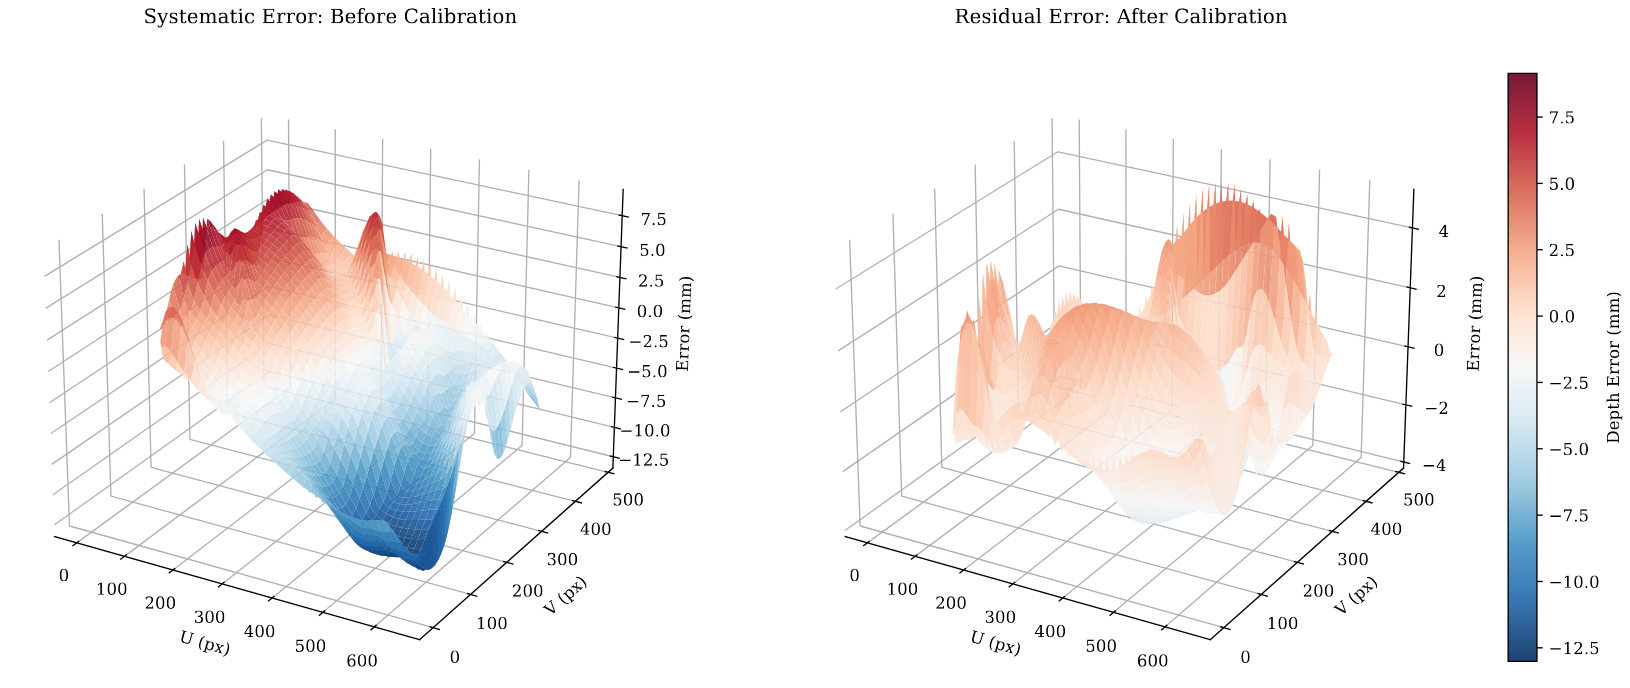
\includegraphics[width=\linewidth]{Figures/chapter3/Camera calibration/spatial_error_comparison_3D.png}
    \caption{Uncalibrated systematic error vs. Residual error after polynomial correction across the image plane ($u, v$).}
    \label{fig:spatial_comparison}
\end{figure}



\subsubsection{Statistical Error Analysis}
To evaluate the stability and precision of the model, error bars and boxplots were generated from the test dataset. Figure~\ref{fig:error_distribution} shows the reduction in variance, confirming that the polynomial model successfully centralized the error around the zero-mean.

\begin{figure}[H]
    \centering
    % Top Subfigure
    \begin{subfigure}{\textwidth}
        \centering
        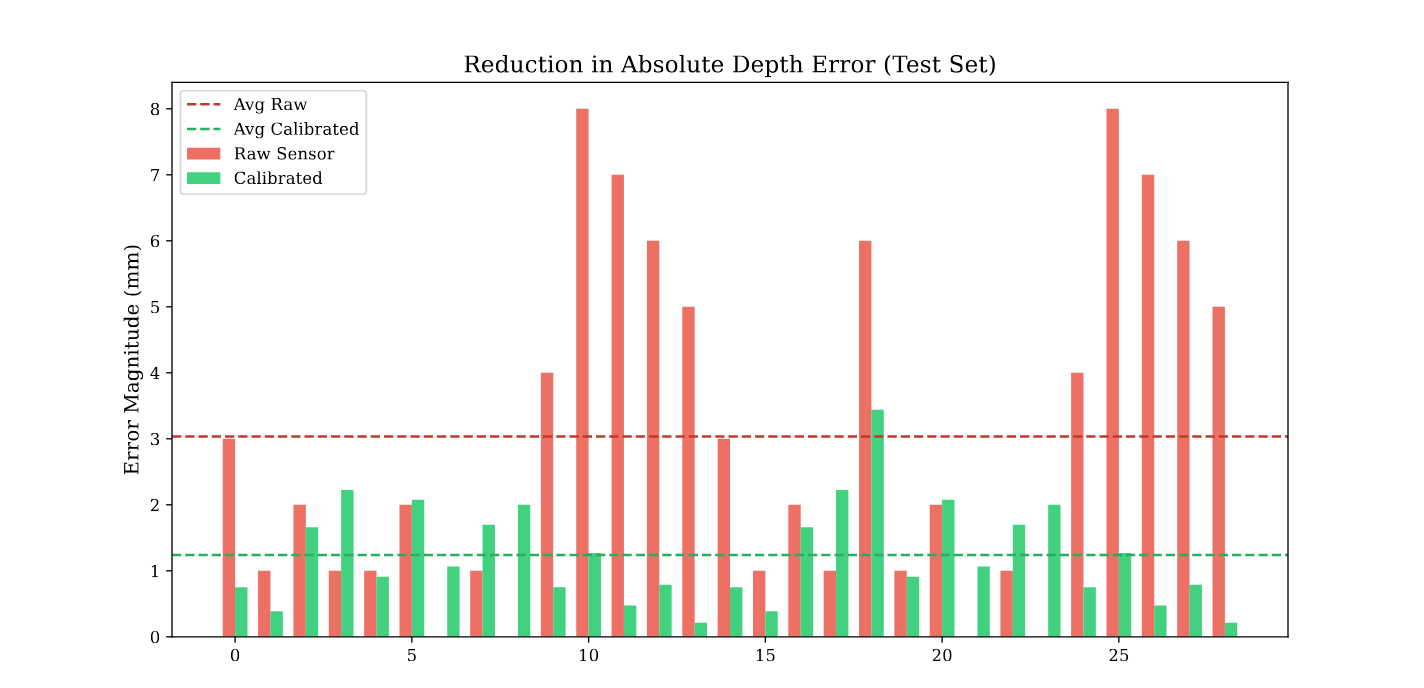
\includegraphics[width=1\textwidth]{Figures/chapter3/Camera calibration/thesis_error_bars.png}
        \caption{Error bars analysis} % Added sub-caption for clarity
    \end{subfigure}
    
    % Bottom Subfigure (Centered)
    \begin{subfigure}{0.6\textwidth} % Matches the image width for tighter centering
        \centering
        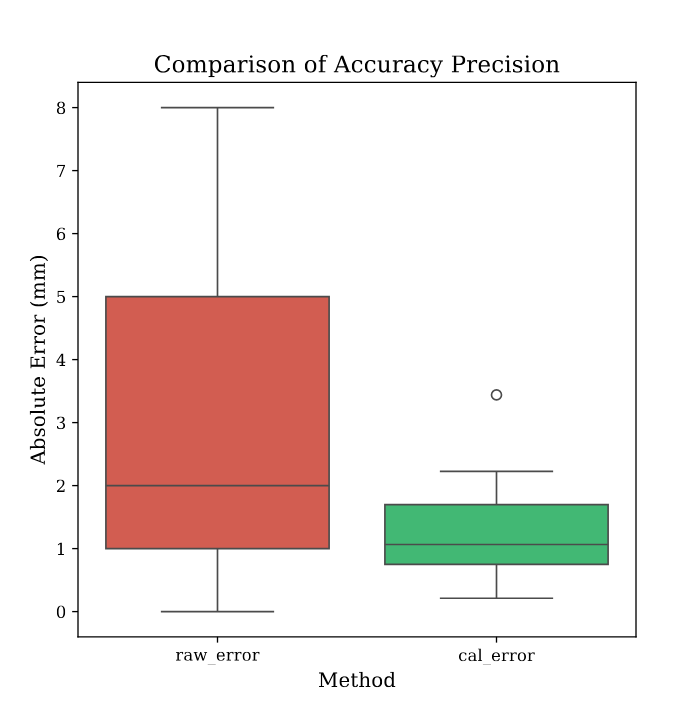
\includegraphics[width=\textwidth]{Figures/chapter3/Camera calibration/thesis_error_boxplot.png}
        \caption{Boxplot of residuals}
    \end{subfigure}
    
    \caption{Error bars and boxplot analysis of depth residuals.}
    \label{fig:error_distribution}
\end{figure}

\subsubsection{Quantitative Performance Metrics}
The quantitative improvement is summarized in Tables~\ref{tab:final_results_train} and~\ref{tab:final_results_test}. These values were extracted from the training and testing logs during model validation.

\begin{table}[H]
\centering
\caption{Quantitative Depth Accuracy Training Results}
\label{tab:final_results_train}
\renewcommand{\arraystretch}{1.2}
\begin{tabular}{|l|c|c|c|}
\hline
\textbf{Metric} & \textbf{Raw Sensor (mm)} & \textbf{Polynomial Model (mm)} & \textbf{Improvement} \\ \hline
MAE             & 4.7857        & 1.1724          & 75.50\%                \\ \hline
RMSE            & 5.5742       & 1.5176            & 72.77\%                \\ \hline
Max Error       & 12.000       & 3.7240             & 68.97\%               \\ \hline
\end{tabular}
\end{table}

\begin{table}[H]
\centering
\caption{Quantitative Depth Accuracy Testing Results}
\label{tab:final_results_test}
\renewcommand{\arraystretch}{1.2}
\begin{tabular}{|l|c|c|c|}
\hline
\textbf{Metric} & \textbf{Raw Sensor (mm)} & \textbf{Polynomial Model (mm)} & \textbf{Improvement} \\ \hline
MAE             & 3.0345        & 1.2407          & 59.11\%                \\ \hline
RMSE            & 3.9741       & 1.4520            & 63.46\%                \\ \hline
Max Error       & 8.0000       & 3.4396             & 57.00\%               \\ \hline
\end{tabular}
\end{table}

\subsubsection{Temporal Stability via Kalman Filtering}
The integration of the Kalman Filter significantly improved the precision of the system for real-time grasping. Figure~\ref{fig:kalman_plot} demonstrates the jitter reduction on a static object.

\begin{figure}[H]
    \centering
    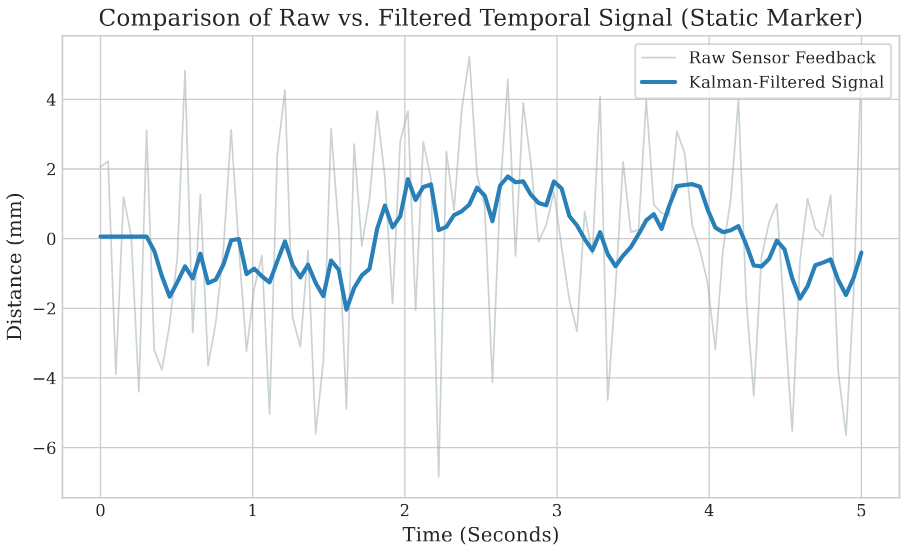
\includegraphics[width=0.9\textwidth]{Figures/chapter3/Camera calibration/thesis_kalman_filter.png}
    \caption{Comparison of raw depth jitter vs. Kalman-filtered output.}
    \label{fig:kalman_plot}
\end{figure}